\documentclass[titlepage]{article}
\usepackage{school-style-packages}
\usepackage[cc]{titlepic}

\begin{document}
\title{Developer's Guide for PINSPEC}
\titlepic{
\includegraphics[width=\textwidth]{images/pinspec.png}}
\maketitle

\section{Introduction}
\subsection{Python vs. SWIG vs. C++}
Fig.~\ref{high-level} illustrates the three major components of PINSPEC: the python codes, the SWIG interface, and the C++ source codes. More specifically, here is the flow of a typical simulation:
\begin{itemize}
\item Users inputs data in a python file;
\item PINSPEC python source codes processes input data, perform Doppler Broadening of the cross sections if requested;
\item SWIG passes the info from python to C++;
\item C++ contains the actualy Monte Carlo kernel, and neutrons are simulated here;
\item If any plotting is requested, generated results would be passed from C++ back to python using SWIG again and python would generate plots. 
\end{itemize}

\begin{figure}[h]
  \centering
  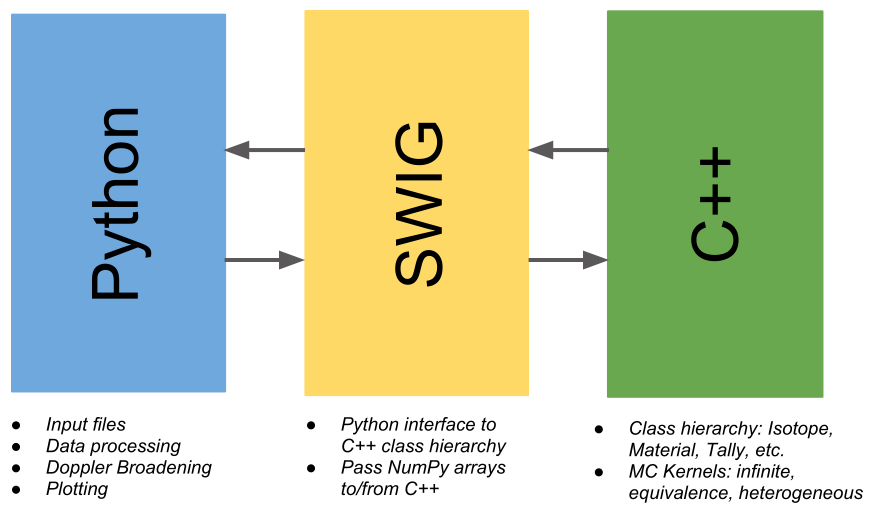
\includegraphics[width=5in]{images/high-level.png}
  \caption{Python Interfacing C++ Through SWIG} \label{high-level}
\end{figure}


\clearpage
\subsection{Major C++ Classes}
C++ using the following major classes: 
\begin{itemize}
\item Geometry: the umbrella class that knows the \# neutrons per batch, \# batches, \# threads, the type of geometry (infinite, infinite equivalent, or heterogeneous) etc. 
\item Region: a region object knows its name, material type, region type, volume and buckling. More specifically, we support 6 types of regions: 
  \begin{itemize}
    \item Infinite medium: this region covers an infinite space. 
    \item Equivalent fuel: this region is a fuel region using the infinite equivalence model. 
    \item Equivalent moderator: this region is a moderator region using the infinite equivalence model. 
    \item Bounded fuel: this region is a fuel region using the true heterogeneous model. 
    \item Bounded moderator: this region is a moderator region using the true heterogeneous model. 
    \item Bounded general: this region is a generalized region bounded by surfaces and is used in the true heterogeneous model. 
  \end{itemize}

\item Surface: Surface objects are used to bound a region. For instance, a surface object knows its name, ID \#, its surface type (x-plane, y-plane, z-cylinder), and its boundary condition (reflective, vacuum, interface). 

\item Material: an material object contains one or more isotope objects, and an material object is used to filled a region object. A material object knows basic info like its name, ID \#, material density, 


\item Isotope:

\item Neutron

\item Tally
\end{itemize}

\clearpage
\subsection{Hierarchy Diagram}
In this section we go more in depths into some of the above classes to illustrate their hierarchy. 

\clearpage
\section{Installation and How To Run} 
An overview of the installation procedures can be found on the users' guide. 



\clearpage
\subsection{Python 2.7 Is The Way to Go!}



\clearpage
\section{Additional Source Code Explanation}
On top of comments in the source code and Doxygen generated files, this section provides some additional information about the source code. 


\clearpage
\subsection{Tally Arithmetic and Operator Overload}
There are three tally arithmetics: 
\begin{enumerate}
\item tally1 + tally2: creates a new tally with the correct statistics. 
\item tally1 + 3.5:
\item tally1.addFloats(numpy.array([1,2])), or addIntegers, or addDoubles. 
\end{enumerate}





\clearpage
\section{Manipulating Python Inputs}
\subsection{Example: Add A New Isotope}

\clearpage
\subsection{Example: Add A New Cross Section}







\clearpage
\section{Manipulating C++ Codes}
\subsection{Create A New Source File}
If you create a new source file, make sure you add it to \textit{setup.py}

\begin{itemize}
\item If you need to pass data from the python input file into the C file, or you would like to retrieve the results generated by C++ and plot or print it using python, see Section~\ref{data}. 
\item Make sure you update the doxygen commenting accordingly, and run doxygen by:
\begin{verbatim}
 doxygen docs/Doxyfile
\end{verbatim}
See more details in Section.~\ref{doxygen}. 

\item If you add in any additional functions, it is nice to update the test suites accordingly. 

\item Two examples are shown about how to add a new tally and a new surface. 
\end{itemize}

\subsection{Passing Data Between Python and C++} \label{data}
If you would like to gain access to an array of data, you need to do so through SWIG. Examples can be found in Geometry.i which contains numpy template. 


\subsection{Doxygen Commenting} \label{doxygen}
To generate html and pdf from source code commenting, run Doxygen by the following command:
\begin{verbatim}
 doxygen docs/doxygen/Doxyfile
\end{verbatim}

If you modify the source code, please update the Doxygen commenting accordingly. For instance, here are some styling suggestions:
\begin{enumerate}
\item For any class structure (including super-class and sub-class), use @class followed by class name, header file name, and header file path. Examples:
\begin{verbatim}
@class Surface Surface.h "pinspec/src/Surface.h"
@class XPlane Surface.h "pinspec/src/Surface.h"
@class YPlane Surface.h "pinspec/src/Surface.h"
\end{verbatim}
In the above examples, Surface is the super-class, and XPlane and YPlane are sub-classes. 

\item For any structure, try using @brief followed by a one-line short description, as well as @details followed by a longer description if needed. 

\item For any structure, use @param followed by parameter name and description to comment on the inputs of a method, and use @return followed by variable name and description to comment on the outputs of a method. 
\end{enumerate}


\clearpage
\subsection{Update Test Suites}

\clearpage
\subsection{Example: Implement A New Surface}

\clearpage
\subsection{Example: Implement A New Tally}


\clearpage
\subsection{Example: Implement A Monte Carlo Variance Reduction Technique}
The main kernel that performs the Monte Carlo simulation is contained in Geometry.cpp as runMonteCarloSimulation(). 

\begin{algorithm}

\caption{High Level Monte Carlo Kernel}
\begin{algorithmic}
\FOR{each batch}
\FOR{each neutron inside the batch}
\STATE Initialize neutrons:

\ENDFOR
\ENDFOR
\end{algorithmic}
\end{algorithm}

\end{document}
